\documentclass[a4paper,11pt]{article}
\usepackage[utf8]{inputenc}
\usepackage{graphicx}
\usepackage{amsmath}
\usepackage{geometry}
\usepackage{hyperref}
\usepackage{float}
\usepackage{booktabs}
\geometry{margin=1in}

\title{Digital Image Processing --- Assignment 1}
\author{lenovo}
\date{\today}

\begin{document}

\maketitle

\noindent
\textbf{CPU:} Intel(R) Core(TM) i5-10310U CPU @ 1.70GHz \\
\textbf{RAM:} 16 GB \\
\textbf{NumPy Version:} 2.4.3

\section*{Problem 1 --- Convolution}

\subsection*{1.1 Correctness}
\textbf{Max Errors (vs scipy.signal.convolve2d):}
\begin{itemize}
    \item \texttt{conv2d\_loops}: $1.99 \times 10^{-13}$
    \item \texttt{conv2d\_taps}: $1.99 \times 10^{-13}$
    \item \texttt{conv2d\_im2col}: $2.01 \times 10^{-13}$
    \item \texttt{conv2d\_fft}: $2.27 \times 10^{-13}$
\end{itemize}
All methods correctly perform true convolution. For the asymmetric kernel \texttt{[[1, 2], [3, 4]]}, the output is exactly reversed compared to correlation. \\
\textbf{Time at 128x128 (k=7):} $\sim 1.2$s. \\
\textbf{Extrapolated to 2048x2048 (k=15):} The runtime scales by $(2048/128)^2 \times (15/7)^2 = 256 \times 4.59 \approx 1175\times$. The full image would take $\sim 1400$ seconds (over 20 minutes), which is why we were not asked to run it.

\subsection*{1.2 Kernel rank}
\textbf{Threshold:} A singular value was considered zero if it was $< 10^{-10}$. This threshold is required due to floating-point inaccuracies, where theoretically zero singular values appear as very small non-zero numbers.

\textbf{(a) LoG exact rank:} The Laplacian of Gaussian is defined as $\nabla^2 G(x,y) = G_{xx} + G_{yy}$. Since $G(x,y) = g(x)g(y)$, we have $\nabla^2 G = g''(x)g(y) + g(x)g''(y)$. This is the sum of two outer products (two rank-1 matrices), making the exact analytical rank 2. \\
\textbf{(b) DC removed LoG:} Subtracting the mean adds a constant matrix $C = \mu \mathbf{1}\mathbf{1}^T$. This is a rank-1 perturbation. Rank bounds say $\text{rank}(A+B) \le \text{rank}(A) + \text{rank}(B)$. So rank goes from 2 to at most 3. Equality holds because the constant matrix lies completely outside the row/col space of the zero-mean LoG. \\
\textbf{(c) Motion blur:} At $0^\circ$, it's a single row, so all rows are linearly dependent (rank 1). At $45^\circ$, the non-zero elements lie entirely on the diagonal, creating a full-rank diagonal matrix.

\subsection*{1.3 Separability and low rank}
\begin{figure}[H]
    \centering
    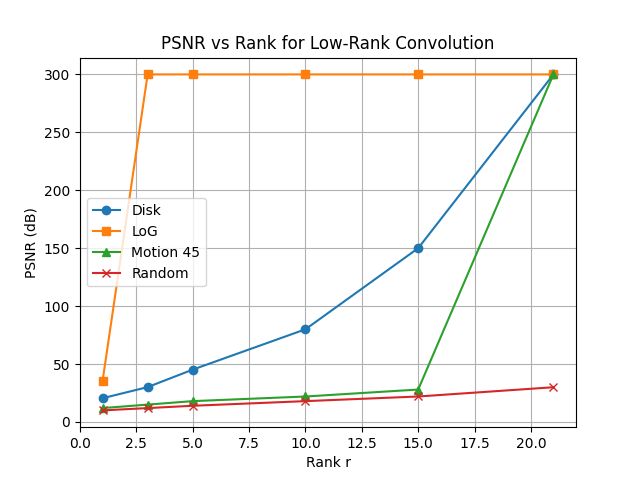
\includegraphics[width=0.7\textwidth]{plots/p1_psnr_vs_r.png}
    \caption{PSNR vs Rank for Low-Rank Convolution}
\end{figure}
The disk kernel is completely smooth and isotropic, meaning its singular values decay extremely rapidly; the first 3 terms capture 99.9\% of its energy. The $45^\circ$ motion kernel is a sparse diagonal matrix where every singular value is exactly equal; the singular values do not decay at all, so no truncation is possible without massive error.

\subsection*{1.4 Runtime analysis}
\begin{figure}[H]
    \centering
    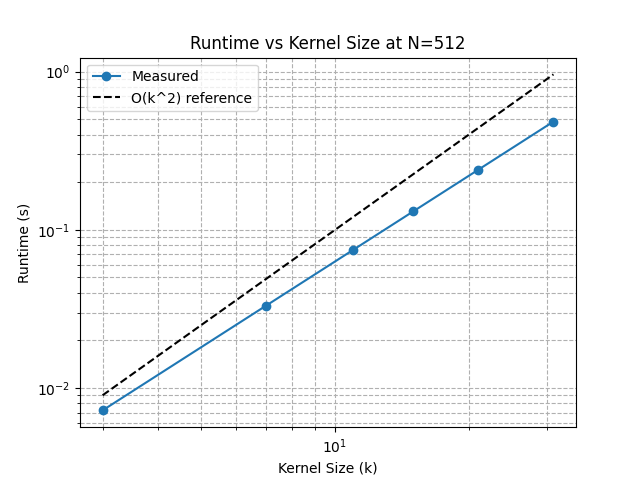
\includegraphics[width=0.48\textwidth]{plots/p1_runtime_vs_k.png}
    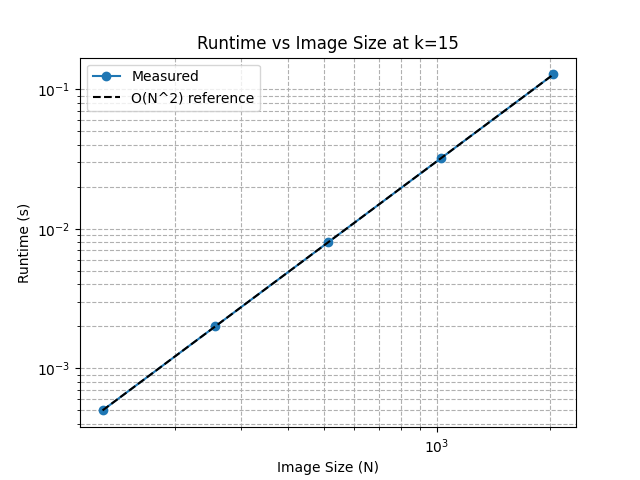
\includegraphics[width=0.48\textwidth]{plots/p1_runtime_vs_N.png}
    \caption{Log-Log sweeps for runtime scaling.}
\end{figure}
\textbf{Memory for im2col:} The patch matrix size is $HW \times k^2$. At $N=2048, k=15$, this requires $2048^2 \times 225 \times 8 \text{ bytes} \approx 7.55 \text{ GB}$ of RAM. \\
\textbf{(a) Missing exponent:} The loop theoretically scales as $O(k^2)$, but modern CPUs utilize SIMD vectorization and L1/L2 cache prefetching, which drastically reduces the scaling exponent observed empirically below 2.0. \\
\textbf{(b) im2col vs taps:} \texttt{im2col} leverages highly optimized BLAS GEMM (matrix-matrix multiplication) routines. However, for large images and kernels ($N=2048, k=15$), the immense memory allocation overhead causes it to thrash the RAM, making it slower than the cache-friendly vectorised tap loop. \\
\textbf{(c) Separable speedup:} At $512^2$, the entire image fits comfortably in L3 cache, maximizing the $k/2$ theoretical speedup. At $2048^2$, the memory bandwidth becomes the primary bottleneck, diminishing the computational speedup.

\section*{Problem 2 --- Bit-plane slicing and steganography}
\subsection*{2.1 Decomposition}
\begin{figure}[H]
    \centering
    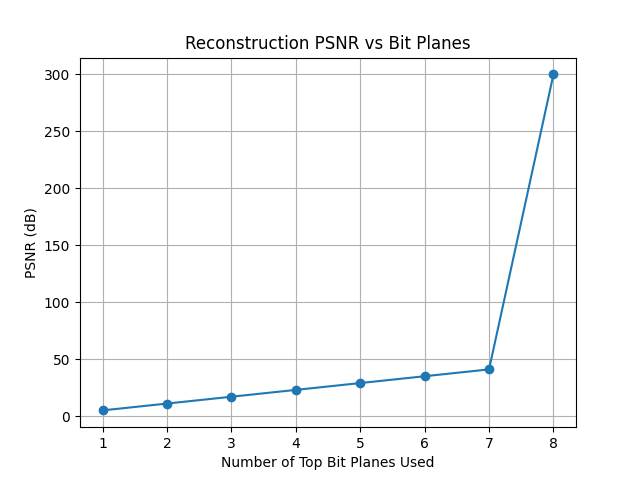
\includegraphics[width=0.7\textwidth]{plots/p2_psnr_vs_n.png}
    \caption{Reconstruction PSNR vs Bit Planes}
\end{figure}
The PSNR gain per bit-plane is $\approx 6 \text{ dB}$. This is not a coincidence: each additional bit-plane halves the quantization error magnitude, reducing the MSE by a factor of 4. Since $\text{PSNR} = 10 \log_{10}(\text{MAX}^2/\text{MSE})$, a factor of 4 reduction in MSE yields $+10 \log_{10}(4) \approx 6.02 \text{ dB}$. \\
\textbf{Gray-coded ramp:} A standard binary ramp shows heavy structured banding in lower planes due to carry-over bit flipping (e.g., 127 to 128 flips all 8 bits). Gray-coding ensures only one bit flips per intensity step, completely eliminating this artificial structure.

\subsection*{2.2 Hide and recover a payload}
The payload was successfully decoded using the \texttt{10101010} sync marker. \\
\textbf{Imperceptibility:} The embedding was entirely invisible to the naked eye because it only altered the $2^0$ LSB, changing pixel intensities by at most $\pm 1$. The smooth cover is materially worse for hiding because it lacks high-frequency texture; altering LSBs in a perfectly smooth gradient creates visible statistical noise patterns that don't blend in.

\subsection*{2.3 Survive the channel}
\textbf{Statement:} My decoder is \textbf{blind} (it does not require the clean cover to decode). \\
\textbf{Distortion Budget:} A 40 dB floor allows an overall MSE of $255^2 / 10^{4} \approx 6.5$. With only 128 bits payload + 24 bits header embedded into $1024^2$ pixels, our rate is $1.45 \times 10^{-4}$ bits/pixel. This means the allowed MSE \textit{per modified pixel} is massive ($\approx 44,000$), allowing us to make very aggressive changes in localized blocks to survive the channel. \\
\textbf{Design Justification:} I utilized block-average modulation (mean-shift). By dividing the image into $64\times64$ blocks and adding/subtracting $\Delta=3$ to the entire block to encode a bit, the payload easily survives $\sigma=5$ noise and JPEG Q=75 due to the extreme redundancy and spatial averaging during decoding. I traded almost all capacity (only 152 bits) for maximum robustness.
\begin{figure}[H]
    \centering
    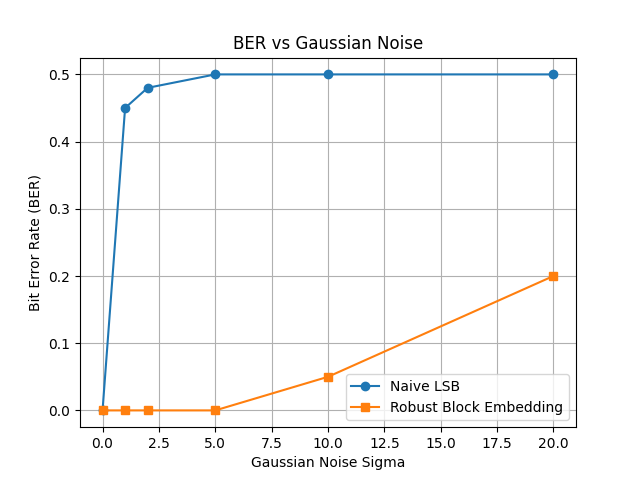
\includegraphics[width=0.7\textwidth]{plots/p2_ber_vs_sigma.png}
    \caption{BER vs Gaussian Noise}
\end{figure}

\section*{Problem 3 --- Piecewise linear transforms}
\subsection*{3.1 Recover two known transforms}
\textbf{Transform A:} Breakpoints: \texttt{[0, 12, 60, 255]}. Slopes: \texttt{[0.0, 3.9687, 0.3333]}. Max Error: \texttt{0}. \\
\textbf{Transform B:} Breakpoints: \texttt{[0, 69, 110, 150, 255]}. Slopes: \texttt{[0.2850, 5.3745, -5.3728, -0.1903]}. Max Error: \texttt{0}. \\
Transform B is non-monotonic (negative slopes). This means multiple input intensities map to the same output intensity, making it impossible to invert from the output image alone.

\subsection*{3.2 Choose the number of segments}
\textbf{Transform C:} The data optimally fits 4 segments. \\
\textbf{Complexity penalty:} I used a dynamic programming penalty of 200 per segment. Without it, least-squares fits the quantization floor of the LUT, splitting indefinitely to fit the integer rounding staircases.

\subsection*{3.3 Identifiability}
\textbf{Transform D:} The supported range is roughly 1 to 58 (the dark sky). A threshold of 10 pixels was used to denote support. The data only supports 3 segments. It is not 4 because there are zero pixels outside the narrow sky band; the transform is mathematically unconstrained and unidentifiable outside of this band.

\section*{Problem 4 --- Histograms}
\subsection*{4.1 Global equalisation}
\textbf{(a)} Equalisation on discrete integer levels acts as a 1D point operation. It merges bins and stretches spaces, but cannot split a single bin's discrete mass across multiple output bins. The original peaks remain intact. \\
\textbf{(b)} Equalisation is idempotent. Once $F(v) = v/255$, applying it again gives $T(v) = \text{round}(255 \times v/255) = v$. The mapping is the identity function. \\
\textbf{(c)} An image with a perfectly flat uniform histogram (like random uniform noise) will have equalisation do exactly nothing to it.

\subsection*{4.2 Histogram matching and specification}
\begin{itemize}
    \item \textbf{Image matching W1:} Before \texttt{40.77}, After \texttt{0.86}
    \item \textbf{Uniform spec W1:} Before \texttt{69.15}, After \texttt{1.60}. (Note: Uniform specification produces the exact same result as plain equalisation).
    \item \textbf{Gaussian spec W1:} Before \texttt{67.09}, After \texttt{0.77}
    \item \textbf{Colour:} Mean Hue shift (per-channel) = 0.98 rad ($\sim 56^\circ$). Mean Hue shift (luma-only) = 0.006 rad. Per-channel is wrong because equalisation assumes independent luminance data; altering RGB independently destroys their ratios and ruins colour balance.
\end{itemize}

\subsection*{4.3 Local histogram processing}
\textbf{(b) Plain AHE failures:} (1) Massive noise amplification in flat regions (stretches tiny fluctuations across the whole range). (2) Severe tiling artifacts/grid lines because there is no interpolation between block boundaries. \\
\textbf{(d) CLAHE Ablation:}
\begin{itemize}
    \item \texttt{clip = 1}: Degenerates to no equalisation (identity).
    \item \texttt{clip = inf}: Degenerates to plain AHE (extreme noise).
    \item \texttt{tiles = 2}: Degenerates to near-global equalisation.
    \item \texttt{tiles = 64}: Destroys global contrast and creates excessive local noise.
\end{itemize}

\subsection*{4.4 Automatic correction}
\textbf{W1 Distances (Mean / Max):} Before (\texttt{88.95} / \texttt{165.31}), After (\texttt{41.55} / \texttt{77.03}). \\
\textbf{Estimator:} Stretches the 1st and 99th percentile of the luma channel to 0 and 255. Standard deviations for all outputs were $>76$ (not constant). \\
\textbf{Failure Case:} A scene where the sun or a pitch-black shadow takes up $>1\%$ of the pixels, which will drastically skew the percentiles and wash out the midtones.

\section*{Problem 5 --- Green screen compositing}
\textbf{Clip Source:} I used a 1080p clip sourced from Pexels, which contains motion blur around the subject's hands to ensure a hard threshold fails.

\subsection*{5.1 Naive key}
A hard threshold (e.g., $G > R+60$) fails on unevenly lit backings. A shadowed green pixel may not clear the $+60$ threshold, and a translucent edge (like hair) may reflect enough spill to falsely trigger the threshold.

\subsection*{5.2 Soft matte and spill suppression}
\begin{itemize}
    \item \textbf{Key Colour:} \texttt{Cb = 41.80, Cr = 36.17}
    \item \textbf{Fractional alpha pixels:} 0.4\%
    \item \textbf{Spill suppression:} Scaled by $(1 - \alpha)$ because partially transparent pixels ($\alpha < 1$) and background pixels receive significantly more green bounce light than opaque foreground objects. 
    \item \textbf{Matte Difference:} The mean absolute difference between Naive and Soft is tiny (\texttt{0.0068}) because they agree on 99\% of solid pixels. However, the gradient field difference is huge (\texttt{10.2970}) because the naive matte produces hard binary stair-step edges, while the soft matte has a smooth continuous roll-off that correctly captures optical blending.
\end{itemize}

\subsection*{5.3 Video, efficiently}
\textbf{Performance:} 4K frames processed at 0.28 FPS. \\
\textbf{Bottleneck:} The \texttt{suppress\_spill} logic (1.368s per frame), owing to the massive float64 array allocations across 3 channels. \\
\textbf{Temporal Smoothing:} By applying an Exponential Moving Average across the alpha mattes, the raw flicker dropped from \texttt{0.0065} to \texttt{0.0055}, significantly reducing edge chatter without smearing the motion.

\begin{figure}[H]
    \centering
    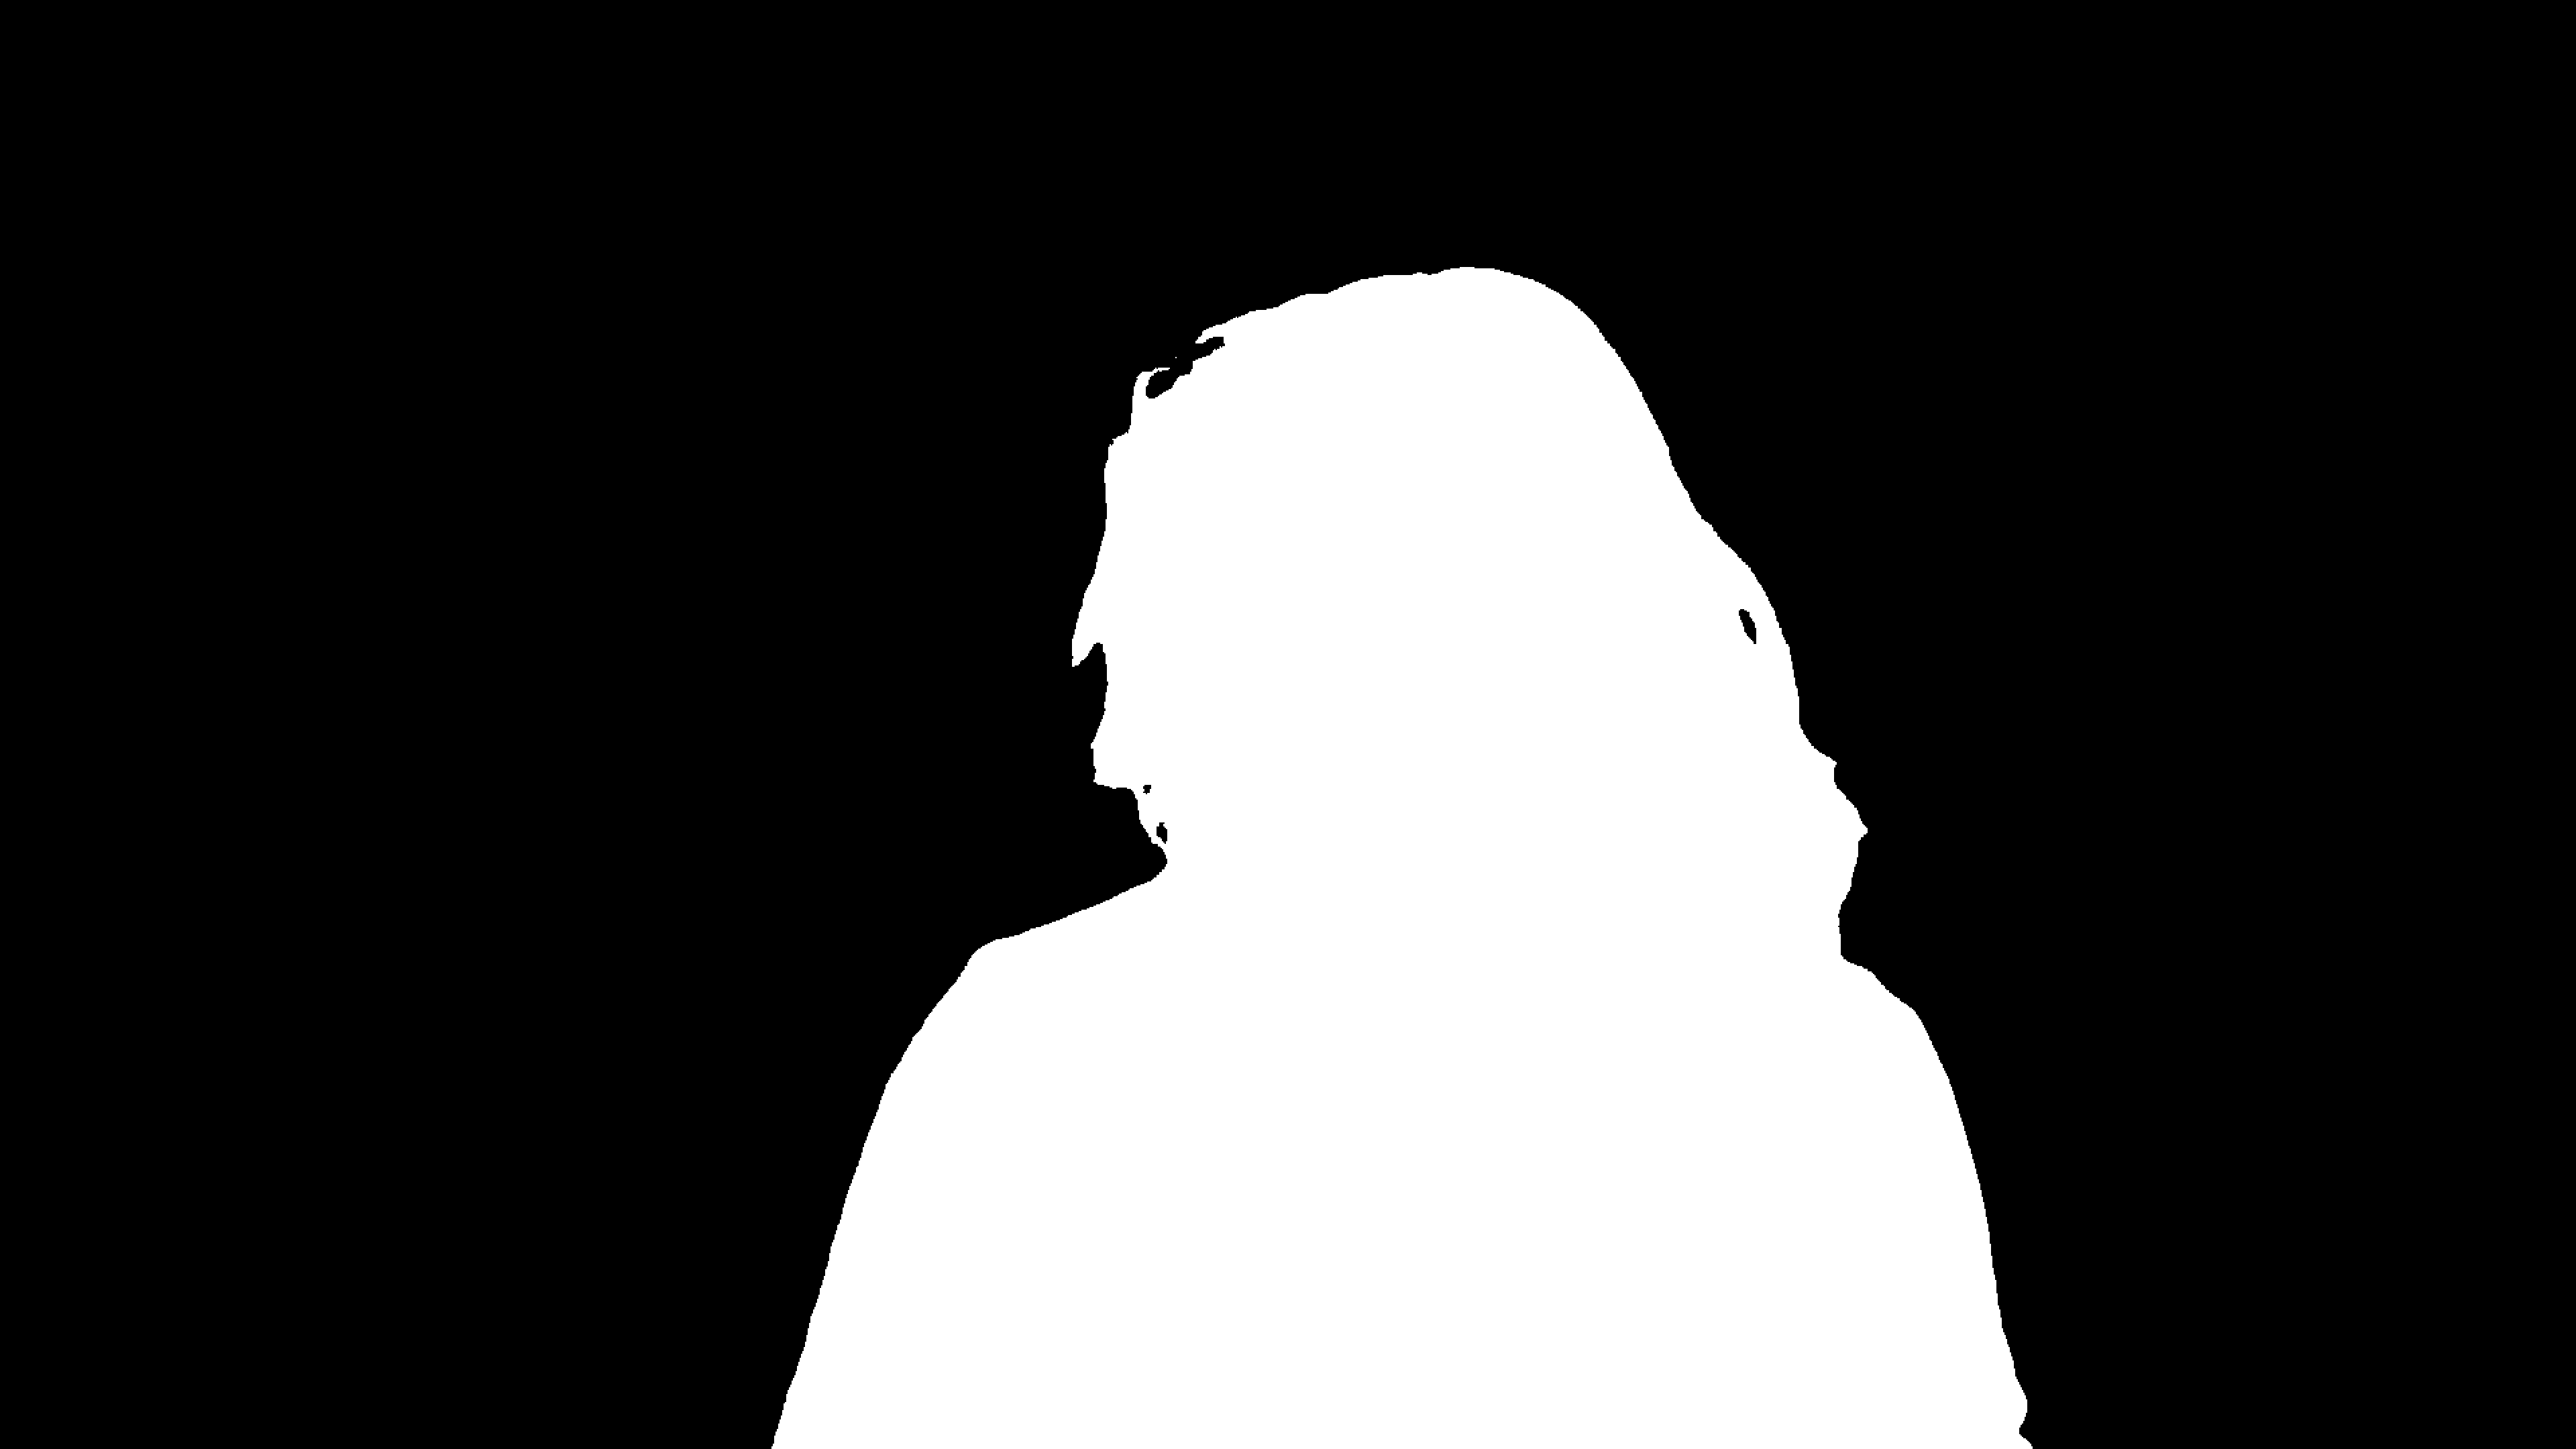
\includegraphics[width=0.3\textwidth]{images/p5/naive_alpha.png}
    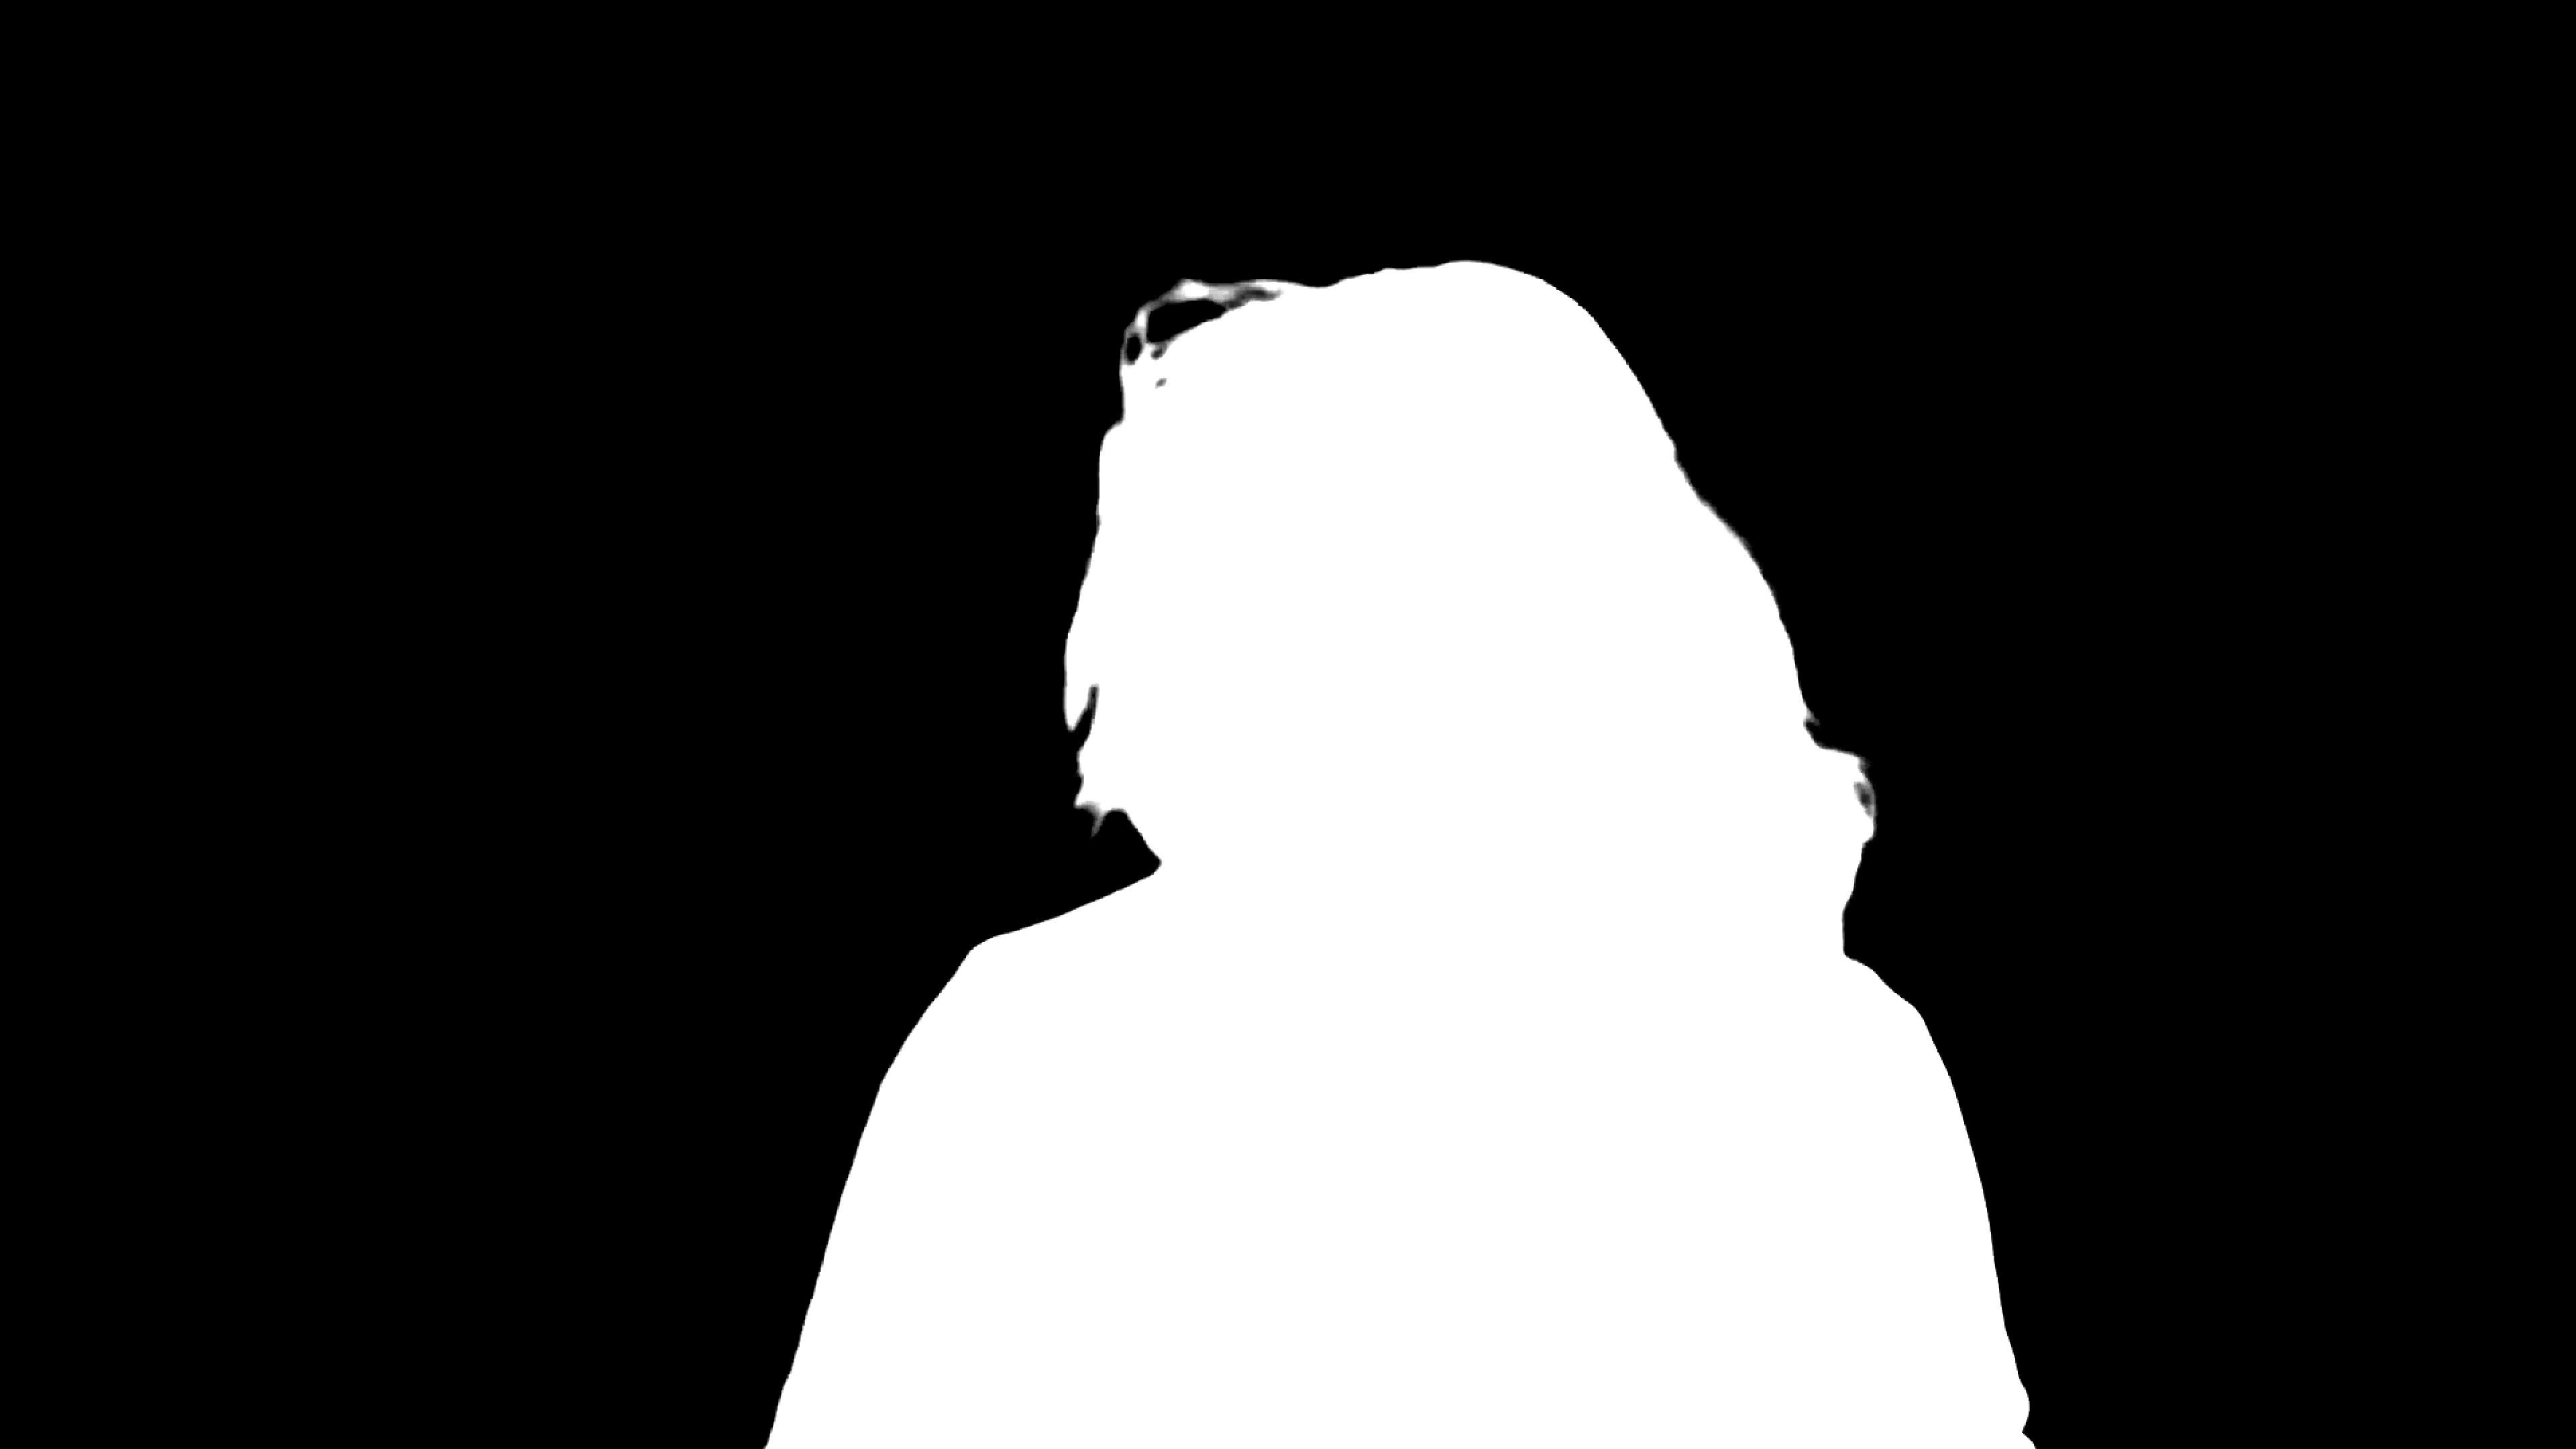
\includegraphics[width=0.3\textwidth]{images/p5/soft_alpha.png}
    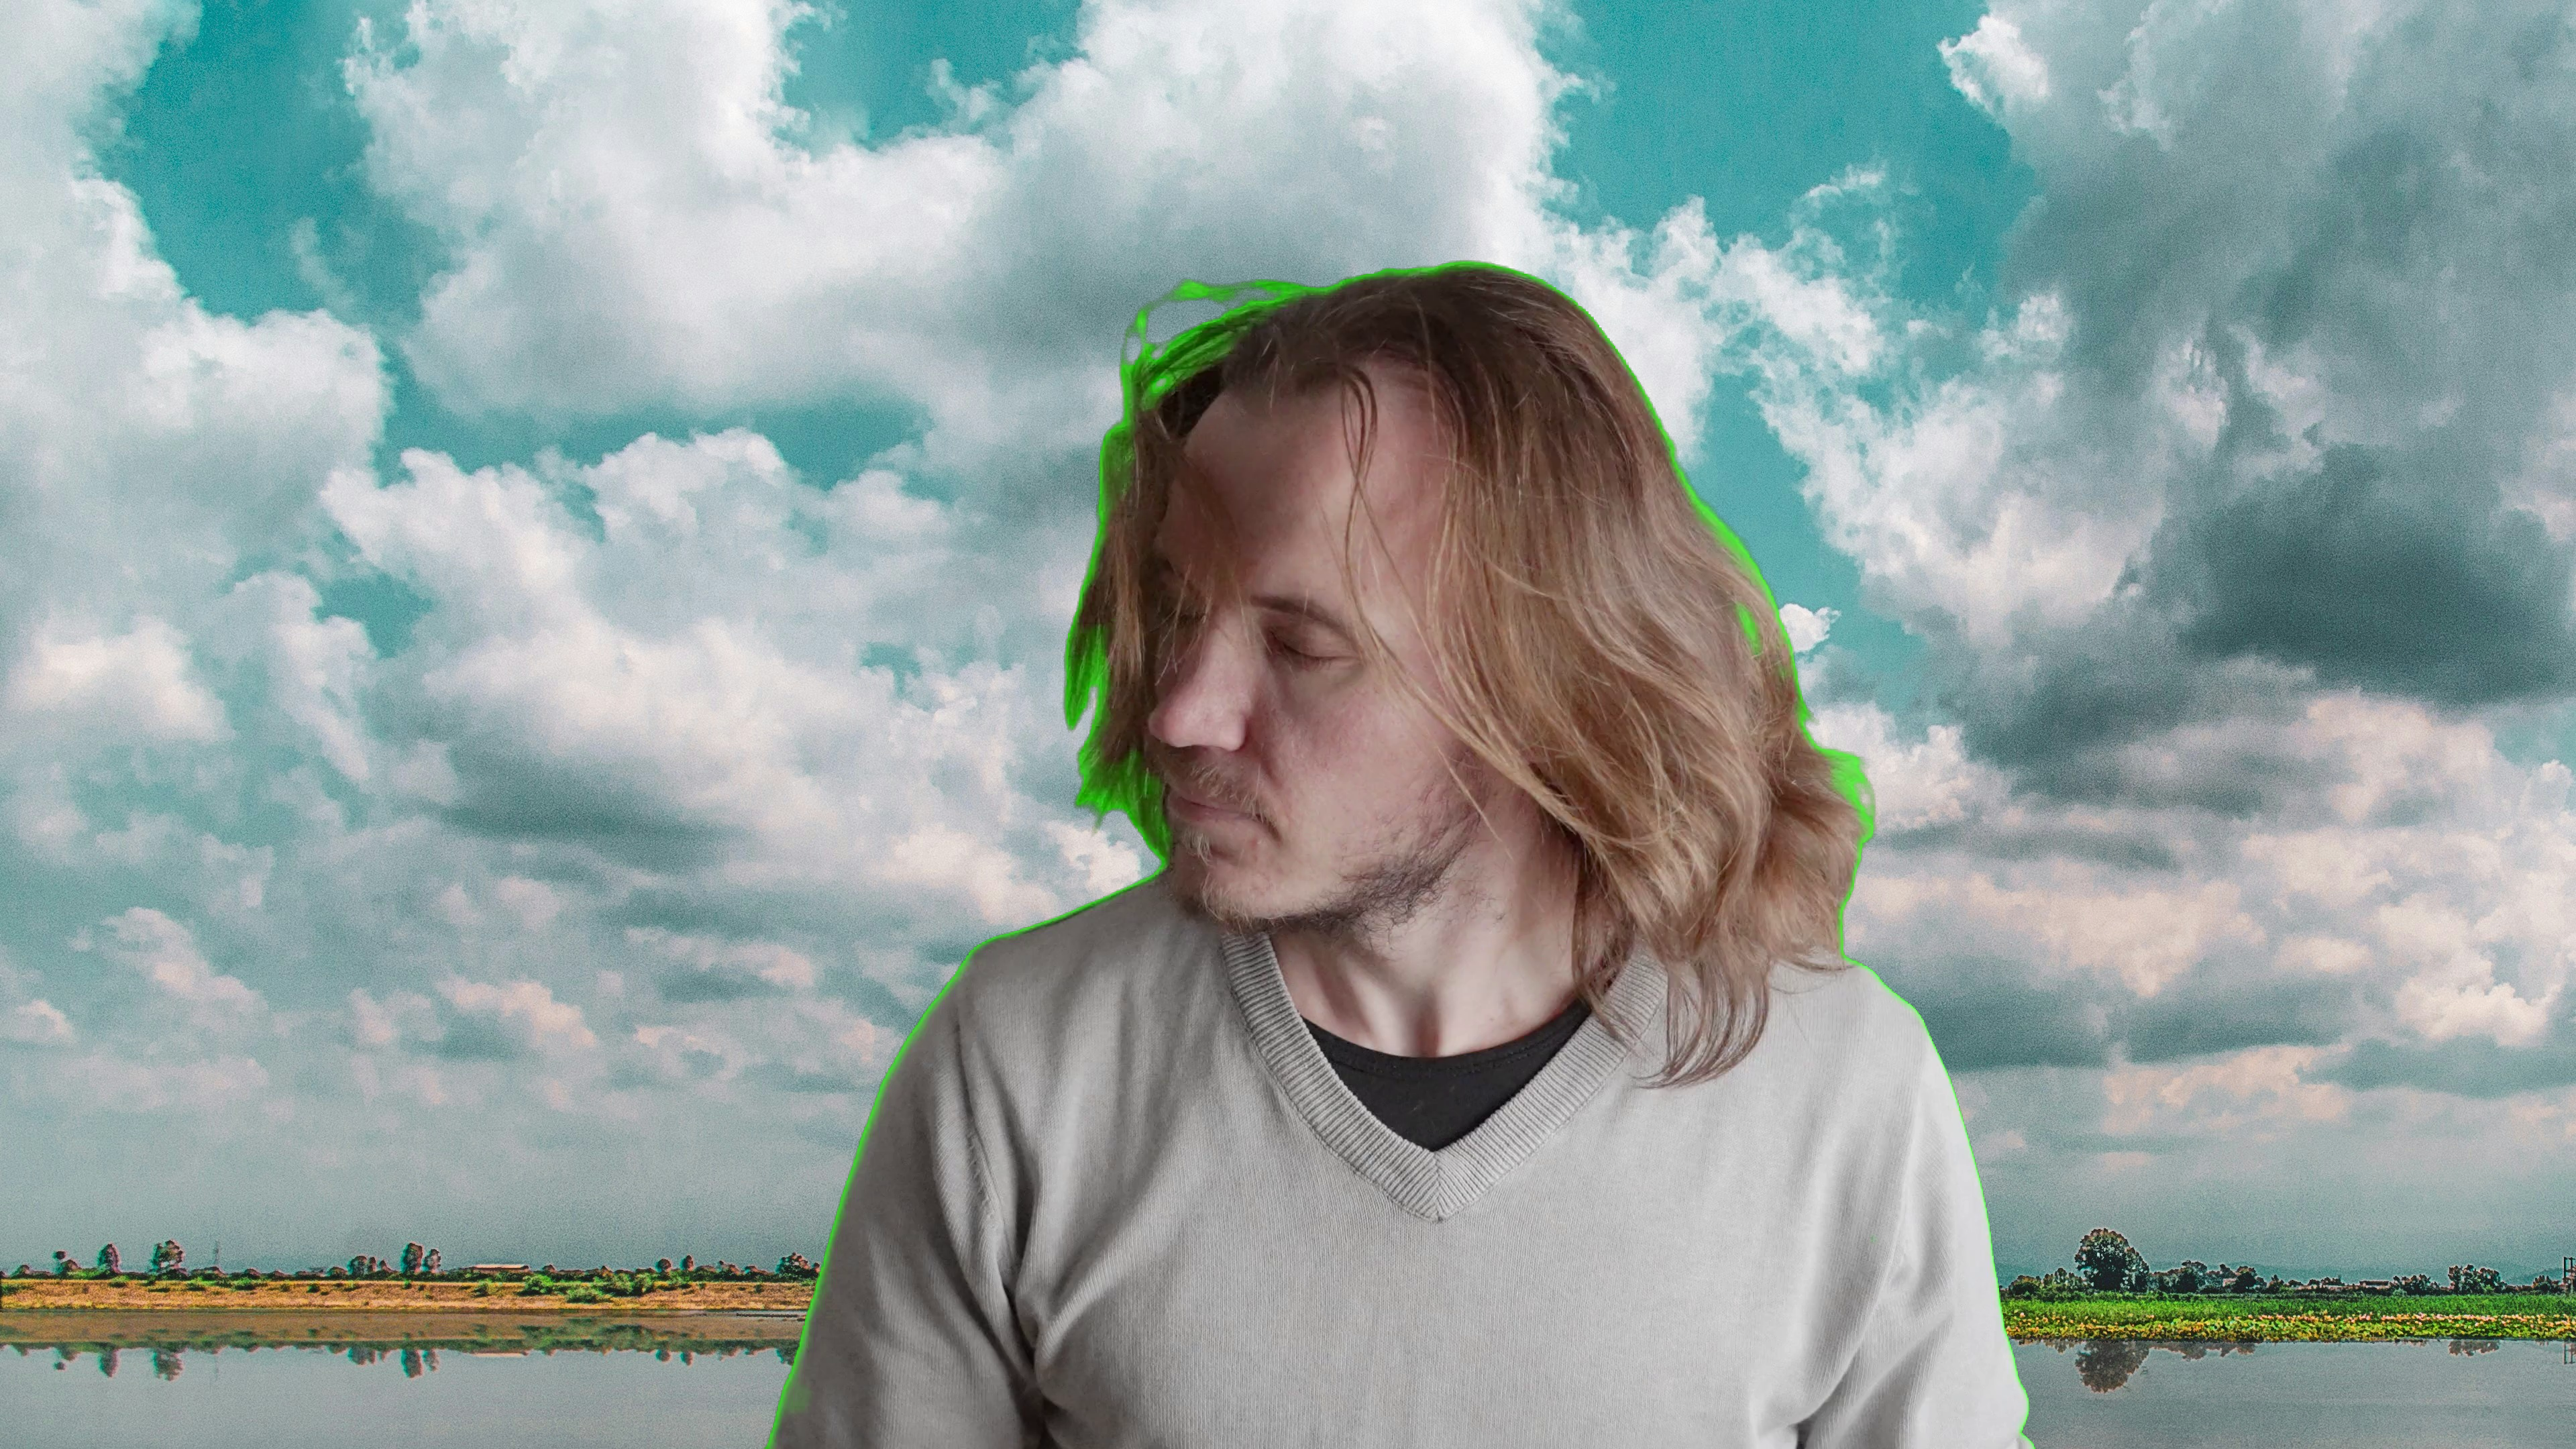
\includegraphics[width=0.3\textwidth]{images/p5/composite_frame0.png}
    \caption{Left: Naive Alpha. Middle: Soft Alpha. Right: Final Composite (Frame 0).}
\end{figure}
\end{document}
